\documentclass[a4paper,14pt]{extarticle}
\usepackage[utf8]{inputenc} % UTF-8 кодировка
\usepackage[russian]{babel} % Русский язык
\usepackage{indentfirst} % красная строка в первом параграфе в главе
\usepackage{amsmath, amsfonts, amssymb, amsthm} % Набор пакетов для математических текстов
\usepackage{cancel} % зачеркивание для сокращений
\usepackage[pdftex]{graphicx} % вставка рисунков
\usepackage{wrapfig, subcaption} % вставка фигур, обтекая текст
\usepackage{caption} % для настройки подписей
\usepackage{tikz} % рисование
\usepackage{circuitikz}
\usepackage{pgfplots} % графики
\usepackage[unicode, pdftex]{hyperref} % гиперссылки
\usepackage{epigraph}
\setlength{\epigraphwidth}{0.45\textwidth}

\usepackage{import}
\usepackage{pdfpages}
\usepackage{transparent}
\usepackage{xcolor}

\newcommand{\incfig}[2][1]{%
    \def\svgwidth{#1\columnwidth}
    \import{./figures/}{#2.pdf_tex}
}

\pdfsuppresswarningpagegroup=1

\title{Завершающее занятие: стандартные поверхности и характеристика Эйлера}
\date{}
\begin{document}
\pagenumbering{gobble}
\maketitle
\vspace{-6em}
\epigraph{В топологии, как и во многих других математических науках, в основном понятия получают свои названия в честь первого ученого, открывшего его после Эйлера}{\textit{Расхожая шутка}}

\section{План}
В каком-то смысле хотим к концу ответить на вопрос о разрешимости задачи о полном двудольном графе с непересекающимися ребрами на различных поверхностях.

Для этого вспомним склеивание как операцию из фактора. Получив из бумаги простейшие поверхности: сферу(=что-угодно, гомеоморфное сфере), ленту Мебиуса, тор(=цилиндр, который при желании можно склеить в тор), можно заметить, что они негомеоморфны друг другу (ПОЧЕМУ?). 

Также мы можем приклеивать эти объекты друг к другу и получать что-то новое. Или не всегда новое?! 

Вот оказывается, что мы получим либо сферу с ручками (каким-то количеством вклеенных торов), либо сферу с пленками (каким-то количеством вклеенных лент Мебиуса). (хороший вопрос, почему пленка, приклеенная к тору, не отличается от одного из таких типов). И снова эти классы негомеоморфны друг другу, а также внутри класса поверхности с разным числом ручек (или пленок) негомеоморфны (ПОЧЕМУ).

А что значит приклеивание ручек или пленок на развертке? И как можно построить сферу с ручками (или пленками) из листа бумаги (если, конечно, обладать навыками сгибать бумагу как угодно). Подсказка: что получится из развертки $abca^{-1}b^{-1}$?

Такое представление поверхностей позволяет легко понимать, что происходит при их разрезании. Попробуйте разрезать ленту Мебиуса посередине. Сделайте новую ленту Мебиуса и разрежьте ее по линии на 1/3 от края. Почему результаты разные? А если то же самое делать для обычного цилиндра или для дважды прокрученной ленты? И еще какие-то случаи из книжки + придумать свою ленту, которая при разрезании даст что-то.

А вот правда ли, что вообще любая замкнутая поверхность является сферой с ручками или с пленками? Оказывается, что да (надеюсь).

Показать процесс разбиения любой поверхности на ручки или пленки.

Вернемся к проблеме двудольного графа. Из тиктока известно, что на плоскости задача не решается. Но, если мы рисуем граф на сфере или на сфере с ручками или пленками. Действует ли там формула Эйлера? Проверьте, к примеру на уже готовых поверхностях из бумаги. 

Оказывается, что есть некоторое число, которое выражает разность из формулы Эйлера --- это Эйлерова характеристика --- и она является топологическим инвариантом. Давайте научимся находить ее значение для стандартных поверхностей (то есть, как мы уже знаем, для всех).

Мы как-то знаем, что у сферы --- это 2. Если мы вырезаем из нее круг, то можно считать его одной из стран графа с одним ребром, которую мы выкинули. Тогда, приклеивание тора добавляет (потом).

То есть Эйлеровы характеристики: $\chi(M_g) = 2-2g$ и $\chi(N_g) = 2-g$. 

Так на каких поверхностях тогда можно решить задачу о двудольном графе? Приведите решение на какой-нибудь из бумажных поверхностей.

\section{Основная часть}
\subsection{Вступление}
Многие скорее всего уже видели задачу с Рис. \ref{graph} в этих ваших тиктоках. И даже большинство успело убедиться, что решить ее невозможно. Но почему? Все дело в теореме, полученной Эйлером, о связи граней, ребер и вершин в графах. Она утверждает В+Г-Р=2.

\begin{figure}[h!]
    \centering
    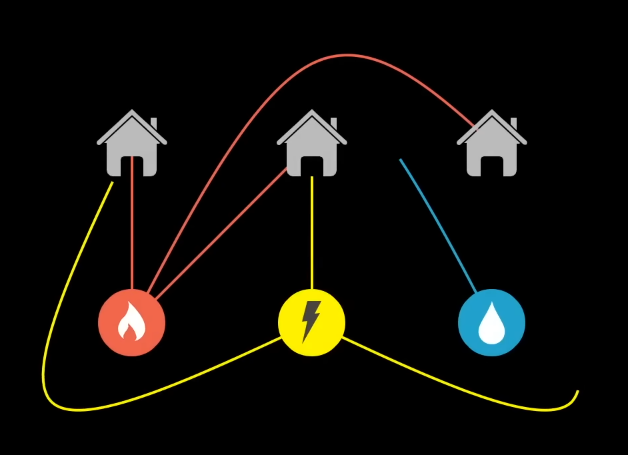
\includegraphics[width=\textwidth]{graph}
    \caption{Интерпретация с канала \textit{3blue1brown}} \label{graph}
\end{figure}

Но ходят слухи, что иногда все же можно решить данную задачу. Просто надо выйти за пределы плоскости. И \textit{3blue1brown} в своем видео предложил пример поверхности, на которой задача решаема. Нам же предстоит разобраться и найти все поверхности, на которых это возможно.

\subsection{Склеивание}
Вообще, мы будем исследовать замкнутые поверхности, то есть какие-то фигуры, получаемые деформированием замкнутого куска плоскости.

Именно поэтому полезно вспомнить про операции стягивания и склеивания. 

Возьмите лист бумаги и попробуйте склеить простейшие поверхности: сферу, тор и ленту Мебиуса. Помните, что нас интересует любые топологически эквивалентные этим пространствам вещи, так что не надо доводить их до идеала. Почему данные поверхности негомеоморфны друг другу? 

А если мы будем приклеивать эти объекты друг к другу, будут ли получаться новые поверхности? Какие есть варианты?

А гомеоморфны ли между собой получающиеся объекты? Почему?

И что значит приклеивание тора к сфере на развертке? А нескольких торов?

\subsection{Разрезание}
А зачем вообще нам с поверхности переходить на развертку? Потому что там легче все анализировать. В частности, из разверток легко понимать, что получится при разрезании каких-то поверхностей.

Возьмите ленту Мебиуса и разрежьте ее посередине. Возьмите еще одну ленту и разрежьте ее теперь, отойдя от края  на треть. Объясните, почему получились разные и именно такие результаты.

\subsection{Любые другие поверхности}
Оказывается, что любая замкнутая поверхность является либо сферой с ручками, либо сферой с пленками. И это круто. Ведь получается, что мы классифицировали всевозможные поверхности. 

Для понимания этого факта можно обратиться к доказательству, которое было первым предложено Джоном Конвеем и носит название ZIP Proof. Во многом такое название пришло из идеи доказательства, которая заключается в разрезании пространства, а потом приклеивании обратно.

\subsection{Эйлерова характеристика поверхностей}
Мы уже обсуждали, что на плоскости задача \ref{graph} не решается. Проверьте на бумажных поверхностях решаемость этой задачи не на плоскости. Как там работает формула Эйлера? Чему равно Г+В-Р? Это то, что называется Эйлерова характеристика $\chi$

Из ваших опытов, вы знаете Эйлеровую характеристику для сферы. Исследуйте, как она меняется меняется при добавлении ручки. И при добавлении пленки.

Выведите формулу Эйлеровой характеристики для сферы с g ручками и для сферы с g пленками.

\subsection{Что там с тиктоком?}
Сделайте вывод, на каких поверхностях задача из тиктока решаема. То есть укажите те поверхности, для которых есть решение, докажите, что для других этих решений нет, и покажите на бумажных версиях поверхностей решения (если такую поверхность можно сложить, конечно).
\end{document}
